\appendix 

\chapter{Review of noise in radio interferometers}
\label{chap:noisereview}

We review in this section the nature of signal and noise in radio interferometry in order to quantitatively understand nature of sky noise and self noise within a unified framework. Our discussion draws on \citet{thompsonmoranswenson, dewey94, kulkarni89,ellingson2011,synthesisimaging}, and aims to clarify the nature of nature of noise in current instruments.

\section{The Radio Sky and Radio Interferometry}
\label{sec:theradiosky}

The radio sky is an angularly and temporally incoherent radiation field\footnote{This description neglects coherent sources such as pulsars or masers which require different noise considerations, but are not of interest in 21\,cm observations.}. In practice, we consider it a continuum of uncorrelated, temporally incoherent point sources which fill the sky with some resolution. For analytic calculation we may assume this resolution to be infinite, while for numerical calculations the resolution will be determined by the length of the longest baseline. 

Let us introduce a real interferometer and consider how it receives such sky emission. Consider an FX correlator\footnote{In an FX correlator, the timestream from each antenna is Fourier transformed (F) first, and then multiplied (X) with those of other antennas.} which forms cross-correlations (known in radio interferometry as \textit{visibilities}) by first sampling the voltage $v_i(t)$ across antenna $i$ at sample frequency $f_s$ over the time period $\Delta T$. Each timestream is Fourier transformed to construct amplitudes $v_i(T,f)$ with frequency resolution $\Delta f=1/\Delta T$ during time window $T=0,\Delta T, 2\Delta T, ...$. The Fourier amplitudes are then cross multiplied with those of other antennas and time-averaged to form the visibility $V_{ij}(f)$,

\begin{equation}
\label{eqn:visdef}
V_{ij}(f)=\frac{1}{N_T}\sum_{T}v_i(T,f)v_j^*(T,f)
\end{equation}
where $N_T=t_\text{obs}\Delta f$ is the total number of measurements of each Fourier mode, $\Delta f$ is the channel bandwidth, and $t_\text{obs}$ is the total integration time.
The temporal coherence of each Fourier component is $1/\Delta f=\Delta T$, and thus samples of $v_i(T,f)$ at successive times are essentially independent\footnote{This constructive model of a radio interferometer is an alternate picture to the quasi-monochromatic plane wave approximation of \citet{synthesisimaging}.}. \textit{This means that we may consider the sky as a continuum of point sources emitting Fourier amplitudes with frequency spacing $\Delta f$, which vary randomly every time $\Delta T$.} 

Having quantified the operation of the FX correlator, we will express the visibility as a function of the sky intensity distribution $I(\theta,\phi)$ and evaluate its mean and variance. We first express the voltage Fourier amplitude across antenna $i$ during time window $T$ as an integral over the electric field Fourier amplitudes $E_0(T,\theta,\phi,f)$ of the continuum of point sources on the sky. These amplitudes are random numbers drawn every $\Delta T$ from a complex Gaussian distribution with variance equal\footnote{In fact, the electric field variance is equal to the intensity only up to a constant of proportionality which in the real world would be absorbed in calibration anyway, we thus neglect it here.} to $I(\theta,\phi)$. Summing over this continuum of sky sources, adding phases accounting for the antenna position on the ground, and adding the receiver noise $n_i(T,f)$, we find
\begin{equation}
\label{eqn:antvoltage}
v_i(T,f) = g\int E_0(\theta,\phi,f)e^{-i\vec{k}\cdot \vec{x}_i}d\Omega+n_i(T,f)
\end{equation}
where $g$ converts from incident electric field in the instrument polarization to voltage and $\vec{k}=\vec{k}(\theta,\phi,f)$. The measured visibility output by the correlator is specified by Eqns. \ref{eqn:visdef} and \ref{eqn:antvoltage}. The mean is given by the ensemble average of $V_{ij}(f)$,
\begin{eqnarray}
\langle V_{ij}(f)\rangle &=&\int\int \langle E_0(\theta,\phi,T,f)E_0^*(\theta',\phi',T,f)\rangle e^{-i(\vec{k}\cdot\vec{x}_i-\vec{k}'\cdot\vec{x}_j)}d\Omega \nonumber \\ 
&&+\delta_{ij}\sigma_\text{rec}^2
\end{eqnarray}
where $\sigma_\text{rec}^2\equiv\langle |n_i|^2\rangle$. Given that emission from different directions in uncorrelated, this reduces to 
\begin{eqnarray}
\label{eqn:vismean}
\langle V_{ij}(f)\rangle &=&\int\langle |E_0(\theta,\phi,T,f)|^2\rangle e^{-i\vec{k}\cdot(\vec{x}_i-\cdot\vec{x}_j)}d\Omega+\delta_{ij}\sigma_\text{rec}^2 \\
&=&\int I(\theta,\phi,f) e^{-i\vec{k}\cdot(\vec{x}_i-\cdot\vec{x}_j)}d\Omega+\delta_{ij}\sigma_\text{rec}^2 
\end{eqnarray}
This integral reduces to a Fourier transform over small fields of view (the van Cittert-Zernicke Theorem), demonstrating that the visibility mean is equal to the Fourier mode of the sky intensity distribution at angular scale $\lambda/|\vec{x}_i-\vec{x}_j|$, with autocorrelation ($i=j$) measurements incurring a receiver noise bias.

Let us now evaluate the variance of the visibility, defined as
\begin{equation}
\sigma_V^2(f)\equiv\langle |V_{ij}(f)|^2\rangle-|\langle V_{ij}(f)\rangle|^2
\end{equation}
where $\langle\rangle$ indicates an ensemble average, in practice equal to a time average over time windows $T$.
Substituting Eqns. \ref{eqn:visdef} and \ref{eqn:antvoltage} into this definition gives
\begin{eqnarray}
\sigma_V^2(f) &=&\frac{1}{N_T^2}\sum_{T,T'}\langle v_i(T,f)v_j^*(T,f)v_i^*(T',f)v_j(T',f)\rangle \nonumber \\
&-&\frac{1}{N_T^2}\sum_{T,T'}\langle v_i(T,f)v_j^*(T,f)\rangle \langle v_i^*(T',f)v_j(T',f)\rangle
\end{eqnarray}

Expanding the 4-product using Wick's theorem gives
\begin{eqnarray}
\sigma_V^2(f)&&=\frac{1}{N_T^2}\sum_{T,T'}[\langle v_i(T,f)v_j^*(T,f)\rangle\langle v_i^*(T',f)v_j(T',f)\rangle \nonumber \\
&&\hspace{18mm}+\langle v_i(T,f)v_i^*(T',f)\rangle\langle v_j^*(T,f)v_j(T',f)\rangle]\nonumber \\
&&-\frac{1}{N_T^2}\sum_{T,T'}\langle v_i(T,f)v_j^*(T,f)\rangle \langle v_i^*(T',f)v_j(T',f)\rangle
\end{eqnarray}
The first term cancels the last term in the equation, and the variance simplifies to
\begin{equation}
\label{eqn:varauto}
\sigma_V^2(f)=\frac{|\langle V_{ii}(f)\rangle|^2}{N_T}
\end{equation}
In summary, the visibility mean and variance are given by
\begin{eqnarray}
\langle V_{i\ne j}(f)\rangle &=&\int I(\theta,\phi,f)e^{-i\vec{k}\cdot(\vec{x}_i-\cdot\vec{x}_j)}d\Omega \label{eqn:vismean}\\
\sigma_V^2(f)&=&\frac{(\sigma^2_\text{sky}(f)+\sigma^2_\text{rec}(f))^2}{N_T} \label{eqn:visvar}
\end{eqnarray}
where $\sigma^2_\text{sky}\equiv\int I(\theta,\phi,f)d\Omega$ is the total received sky power. In the next subsections we will look at the limiting cases of these equations and define the different noise regimes in radio interferometry.

\section{Sky Noise, Self Noise, and Receiver Noise}
\label{sec:skyselfreceivernoise}
The receiver contribution to the variance ($\sigma_\text{rec}^2$) is known as \textit{receiver noise}, and typically dominates at high frequencies as the galactic synchrotron and bremsstrahlung brightness decreases rapidly with frequency. Neglecting real world complications such as cross-talk, receiver noise is uncorrelated between antennas, and can thus be mitigated by adding more antennas.

On the other hand, the contribution to the variance from sky emission ($\sigma_\text{sky}^2)$ is known as \textit{sky noise}. Why is this distinction useful? If the interferometer is sky noise dominated, then we are liberated from needing extremely low noise amplifiers or a very high fidelity impedance match with the sky as we would need in receiver noise dominated instruments. As sky noise results from actual sky emission and not electronics noise, it is not immediately clear whether it is entirely uncorrelated between different antennas, and thus, whether adding antennas improves sensitivity. To determine this, we must consider a last type of noise known as \textit{self noise}. 

The contribution of any sky emission to the visibility variance is known as \text{self noise} if that same emission contributes significantly to the visibility mean (Eqn. \ref{eqn:vismean}). Of course, \textit{any} source of sky emission contributes at \textit{some} level to both the visibility mean and variance, but the notion of sky noise is useful when it contributes a significant fraction of both. Physically this means that the voltage fluctuations across each antenna are dominated by the real emitted signal from the celestial source dominating the visibilities. But if that is the case then why is there any noise whatsoever in the visibility measurement? It is easy to understand the reason in the context of single dish measurements. Because the source emission is fundamentally stochastic, its emitted amplitude is a random timestream whose mean equals the true intensity only after infinitely many samples. Self noise may thus be regarded as the \textit{sample variance} on the measured visibilities. 

In a self noise dominated interferometer, adding more antennas provides little new information about the sky as they receive the same (albeit timeshifted) timestream of emission from each celestial source. Adding new antennas of course yields more baselines, but if these new visibilities provide little new information, then their noise must be correlated with those of existing baselines. To quantify this, we compute the covariance $C_{ij,kl}$ between baselines $ij$ and $kl$, defined by
\begin{equation}
C_{ij,kl}\equiv\langle V_{ij}V_{kl}^*\rangle-\langle V_{ij}\rangle\langle V_{kl}^*\rangle
\end{equation}
Evaluating this in the same way we calculate $\sigma_V^2$ in Sec. \ref{sec:theradiosky} results in
\begin{equation}
\label{eqn:covfinal}
C_{ij,kl}=\frac{\langle V_{ik}\rangle\langle V_{jl}^*\rangle}{N_T}
\end{equation}
We see that the covariance between baselines $ij$ and $kl$ is related to the visibilities which would be measured by baselines $ik$ and $jl$. The covariance increases if the distance between these baselines is reduced, or decreased if the distance increases, but it is independent of the length of the baselines themselves.

\begin{figure}[t]
\centering
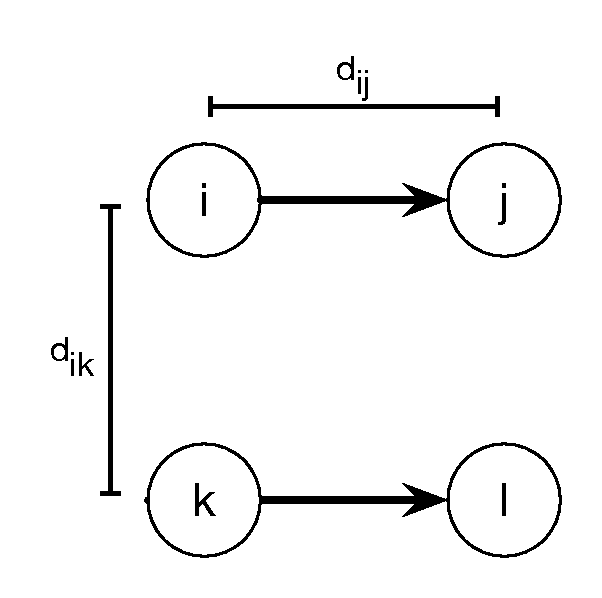
\includegraphics[width=2.5in]{skynoise/array2by2.pdf}
\caption[The level of self noise in baselines is set by their separation.]{The level of self noise in baselines $ij$ and $kl$ is set not by the length of these baselines $d_{ij}$, but by the separation of these baselines from each other $d_{ik}$. }
\label{fig:array2by2}
\end{figure}

This result was first derived by \citet{kulkarni89} for the case of an extremely bright point source which dominates over all other sky emission and receiver noise. In that case, the noise correlation, defined as the ratio of covariance to variance, 
\begin{equation}
\label{eqn:noisecorr}
c \equiv \frac{C_{ij,kl}}{\sigma_V^2}=\frac{|\langle V_{ik}\rangle\langle V_{jl}^*\rangle|}{|\langle V_{ii}\rangle|^2}
\end{equation}
approaches unity, $c=|I_\text{source}e^{-i\vec{k}\cdot(\vec{x}_i-\vec{x}_k)}||I_\text{source}e^{i\vec{k}\cdot(\vec{x}_j-\vec{x}_l)}|/I_\text{source}^2=1$. 
This confirms our intuition that in the self noise regime the noise on different visibilities is strongly correlated, so adding additional antennas does not improve sensitivity. 

Lastly, let us consider the sky noise regime when it is \textit{not} self noise, as is the case in typical low frequency radio interferometers like the MWA. At MWA frequencies (100--200\,MHz), typical sources range from hundreds of mJy to several Jy, whereas the diffuse Galactic emission (dominated by radio synchrotron) has brightness temperature of $\sim200$\,K, translating into a flux density of $2 k_B T_\text{gal}\Omega_\text{FWHM}/\lambda^2\sim2 k_B T_\text{gal}/A\sim30$\,kJy. The noise power sourced by the receiver noise corresponds to an effective brightness temperature of 25--50\,K, subdominant to sky emission. Thus we see that the diffuse Galactic emission dominates the incident power, and thus, the visibility variance. Expressing the flux as a brightness temperature we arrive at the well-known radiometer equation.
\begin{equation}
\sigma_V=\frac{2 k_B T_\text{gal}}{A\sqrt{t_\text{obs}B}}
\end{equation}
But while the diffuse Galactic emission dominates the incident flux, and thus, the visibility variance, its contribution to the mean visibilities is very small. As discussed above, in the flat sky approximation, each visibility measures exactly one mode of the Fourier transform of the sky intensity distribution. The contribution of a constant background to non-zero Fourier modes is thus zero, meaning that the diffuse emission produces no self noise. 

In reality, the diffuse emission is not exactly constant across the sky and the curved sky disturbs the exact Fourier relationship so that even a constant sky background has some leakage into the visibility means. This real diffuse emission will result in some small level of self noise. To quantify this, consider the self-noise induced noise correlation between two parallel baselines positioned as close as possible from each other as in Fig. \ref{fig:array2by2} with $d_{12}=d_{13}=5\,\text{m}$, the size of an MWA tile. Assuming such short baselines are dominated by diffuse emission, the visibility mean is given by $\langle V_{ik}\rangle\sim(2k_BT_\text{gal}/\lambda^2)\int B(\theta,\phi)e^{i\vec{k}\cdot\vec{b}}d\Omega$. The integral is of order $10^{-1.5}$ or smaller over the MWA band, 100--200\,MHz, while $\langle V_{ii}\rangle \sim 2k_BT_\text{gal}/\lambda^2$. Then the noise correlation between the pair of baselines is $c\sim10^{-3}$ at worst. What does a noise correlation of 0.1\% mean? It means that the variance on the average of these two redundant baselines is 0.1\% larger than it would be were their noises independent, an entirely negligible effect. Note that this correlation does not affect how visibility noise averages down with time.

We find a comparable level of noise correlation, 0.1\%, for HERA dishes over the same band, and somewhat larger values of a few percent for PAPER near 100\,MHz. These numbers are worst cases, for physically touching baselines. In real arrays, even the closest antennas are typically placed no closer than of order a wavelength to mitigate cross-coupling, and of course a baseline has very few close neighbor baselines anyway, most other baselines are much farther away. 

%HERA is compact but has negligible sky noise correlation, but maybe that's because it's not electrically compact...should I use ultracompact instead???